% \documentclass[aspectratio=169,notes]{beamer}
\documentclass[aspectratio=169]{beamer}
\usetheme[faculty=phil]{fibeamer}
\usepackage{polyglossia}
\setmainlanguage{english} %% main locale instead of `english`, you
%% can typeset the presentation in either Czech or Slovak,
%% respectively.
\setotherlanguages{russian} %% The additional keys allow
%%
%%   \begin{otherlanguage}{czech}   ... \end{otherlanguage}
%%   \begin{otherlanguage}{slovak}  ... \end{otherlanguage}
%%
%% These macros specify information about the presentation
\title[Artificial Intelligence Software (AIS)]{Artificial Intelligence Software, Lecture 10} %% that will be typeset on the
\subtitle{Web APIs and AI Interfaces: REST, FastAPI, and Gradio
\\ \ \\ \  } %% title page.
\author{Oleg Bulichev}
%% These additional packages are used within the document:
\usepackage{ragged2e}  % `\justifying` text
\usepackage{booktabs}  % Tables
\usepackage{tabularx}
\usepackage{tikz}      % Diagrams
\usetikzlibrary{calc, shapes, backgrounds}
\usetikzlibrary{decorations.pathreplacing,calligraphy,calc,graphs}
\usepackage{amsmath, amssymb}
\usepackage{url}       % `\url`s
\usepackage{listings}  % Code listings
\usepackage{subfigure}
% \usepackage{floatrow}
% \usepackage{subcaption}
\usepackage{mathtools}
\usepackage{todonotes}
\usepackage{fontspec}
\usepackage{multicol}
\usepackage{pdfpages}
\usepackage{wrapfig}
\usepackage{qrcode}
\usepackage{animate}
\usepackage{booktabs}
\usepackage{multirow}
\usepackage{graphicx}
\usepackage{colortbl}

\graphicspath{{resources/}}
\frenchspacing

\setbeamertemplate{caption}{\raggedright\insertcaption\par}
\usetikzlibrary{graphs}
\usetikzlibrary{positioning,arrows.meta}

% \usepackage[backend=biber,style=ieee,autocite=footnote]{biblatex}
% \addbibresource{biblio.bib}
% \DefineBibliographyStrings{english}{%
%   bibliography = {References},}

\newcommand{\oleg}[2][] {\todo[color=red, #1] {OLEG:\\ #2}}
\newcommand{\fbckg}[1]{\usebackgroundtemplate{\includegraphics[width=\paperwidth]{#1}}}%frame background

\usepackage[framemethod=TikZ]{mdframed}
\newcommand{\dbox}[1]{
\begin{mdframed}[roundcorner=3pt, backgroundcolor=yellow, linewidth=0]
\vspace{1mm}
{#1}
\vspace{1mm}
\end{mdframed}
}

\newcommand{\imgmock}[2]{
\fbox{\parbox[c][0.48\textheight][c]{0.92\linewidth}{\centering\textbf{Mock image placeholder}\\[2mm]#1\\[2mm]\footnotesize #2}}
}

\begin{document}
\setlength{\abovedisplayskip}{0pt}
\setlength{\belowdisplayskip}{0pt}
\setlength{\abovedisplayshortskip}{0pt}
\setlength{\belowdisplayshortskip}{0pt}

\fbckg{fibeamer/figs/title_page.png}
\frame[c]{\setcounter{framenumber}{0}
    \usebeamerfont{title}%
    \usebeamercolor[fg]{title}%
    \begin{minipage}[b][6.5\baselineskip][b]{\textwidth}%
        \textcolor{black}{\raggedright\inserttitle}
    \end{minipage}
    % \vskip-1.5\baselineskip

    \usebeamerfont{subtitle}%
    \usebeamercolor[fg]{framesubtitle}%
    \begin{minipage}[b][3\baselineskip][b]{\textwidth}
        \raggedright%
        \insertsubtitle%
    \end{minipage}
    \vskip.25\baselineskip
}
%   \frame[c]{\maketitle}

\fbckg{fibeamer/figs/common.png}

\note{\scriptsize \begin{itemize}
        \item \
    \end{itemize}}

\begin{frame}[t]{Lecture Plan}
\framesubtitle{}
\begin{enumerate}
    \item \textbf{TCP/IP and HTTP} — how the web works under the hood
    \item \textbf{REST API} — design principles and HTTP methods
    \item \textbf{FastAPI} — building REST servers in Python
    \item \textbf{Gradio} — instant web UIs for AI models
    \item \textbf{Putting it together} — exposing a model via FastAPI + Gradio
\end{enumerate}
\vspace{4mm}
\textbf{Extra material (Jupyter notebooks)}:

\texttt{extra\_material/rest\_api\_example.ipynb}

\texttt{extra\_material/gradio\_example.ipynb}
\end{frame}

\begin{frame}[t]{The Internet in Layers}
\framesubtitle{TCP/IP stack overview}
\vspace*{-0.5cm}
\begin{columns}[T,onlytextwidth]
    \begin{column}{0.52\textwidth}
        \begin{enumerate}
            \item \textbf{Link layer} — hardware frame delivery within one network segment (Ethernet, Wi-Fi)
            \item \textbf{Internet layer} — packet routing across networks (IP)
            \item \textbf{Transport layer} — reliable data delivery between hosts (TCP, UDP)
            \item \textbf{Application layer} — structured data exchange between programs (\textbf{HTTP}, FTP, DNS\ldots)
        \end{enumerate}

    \end{column}
    \begin{column}{0.46\textwidth}
        \vspace*{-1cm}
        \begin{figure}[H]
            \centering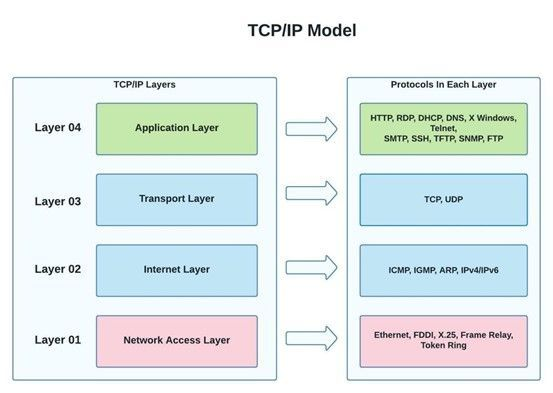
\includegraphics[height=6cm,width=1\textwidth,keepaspectratio]{tcp_ip_layer_diagram.jpg}
            % \caption{caption_name}
            \label{fig:tcp_ip_layer_diagram.jpg}
        \end{figure}
        \vspace*{-1cm}
               {We work at the \textbf{Application layer}. Everything below is handled by the OS and hardware.}
    \end{column}
\end{columns}

\end{frame}

\begin{frame}[t]{HTTP Request and Response}
\framesubtitle{The language of the web}
\vspace*{-0.4cm}
\begin{columns}[T,onlytextwidth]
    \begin{column}{0.49\textwidth}
        \textbf{Request structure}
        \begin{itemize}
            \item \textbf{Request line}: method + URL + version
            \item \textbf{Headers}: metadata (Host, User-Agent, Accept, \ldots)
            \item \textbf{Empty line}
            \item \textbf{Body}: optional data (JSON, form fields, file)
        \end{itemize}
        \vspace{2mm}
        \textbf{HTTP methods}\\
        \texttt{GET} · \texttt{POST} · \texttt{PUT} · \texttt{PATCH} · \texttt{DELETE}
    \end{column}
    \begin{column}{0.49\textwidth}
        \textbf{Response structure}
        \begin{itemize}
            \item \textbf{Status line}: version + \textbf{status code} + message
            \item \textbf{Headers}: Content-Type, Content-Length, \ldots
            \item \textbf{Empty line}
            \item \textbf{Body}: HTML, JSON, binary data, \ldots
        \end{itemize}
        \vspace{2mm}
        \textbf{Status code families}\\
        \texttt{2xx} success · \texttt{3xx} redirect\\
        \texttt{4xx} client error · \texttt{5xx} server error
    \end{column}
\end{columns}
\end{frame}

\begin{frame}[t]{Query Strings and URL Encoding}
\vspace*{-0.4cm}
\begin{columns}[T,onlytextwidth]
    \begin{column}{0.54\textwidth}
        Parameters are appended after \texttt{?} and separated by \texttt{\&}:
        \vspace{1mm}
        \begin{center}
        \footnotesize
        \texttt{https://api.example.com/search?term=hello\&limit=10}
        \end{center}
        \vspace{2mm}
        Only ASCII letters, digits, and a few symbols are safe. Everything else must be \textbf{percent-encoded}:
        \begin{center}
        \footnotesize
        \begin{tabular}{@{}ll@{}}
        \toprule
        Character & Encoded \\
        \midrule
        Space & \texttt{\%20} \\
        \texttt{\&} & \texttt{\%26} \\
        Non-ASCII (e.g.\ ü) & \texttt{\%C3\%BC} \\
        \bottomrule
        \end{tabular}
        \end{center}

    \end{column}
    \begin{column}{0.44\textwidth}
        \centering
        \begin{figure}[H]
            \centering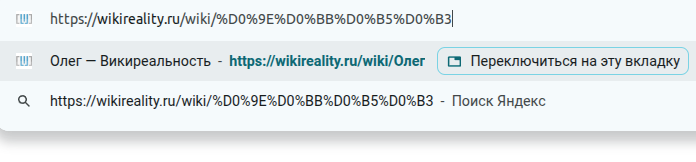
\includegraphics[height=6cm,width=1\textwidth,keepaspectratio]{name_conv.png}
            \label{fig:name_conv.png}
        \end{figure}
    \end{column}
\end{columns}
\end{frame}

\begin{frame}[t]{What Is a REST API?}
\framesubtitle{Representational State Transfer}
\begin{columns}[T,onlytextwidth]
    \begin{column}{0.56\textwidth}
        A \textbf{REST API} is an architectural style for building web services:
        \begin{itemize}
            \item \textbf{Resources} are data objects (user, post, task, \ldots) identified by URIs
            \item \textbf{Standard HTTP methods} define the operation
            \item \textbf{Stateless}: every request is self-contained, no server session
            \item Data exchanged as \textbf{JSON} (typically)
        \end{itemize}
    \end{column}
    \begin{column}{0.42\textwidth}
        \vspace*{-1.5cm}
        \begin{figure}[H]
            \centering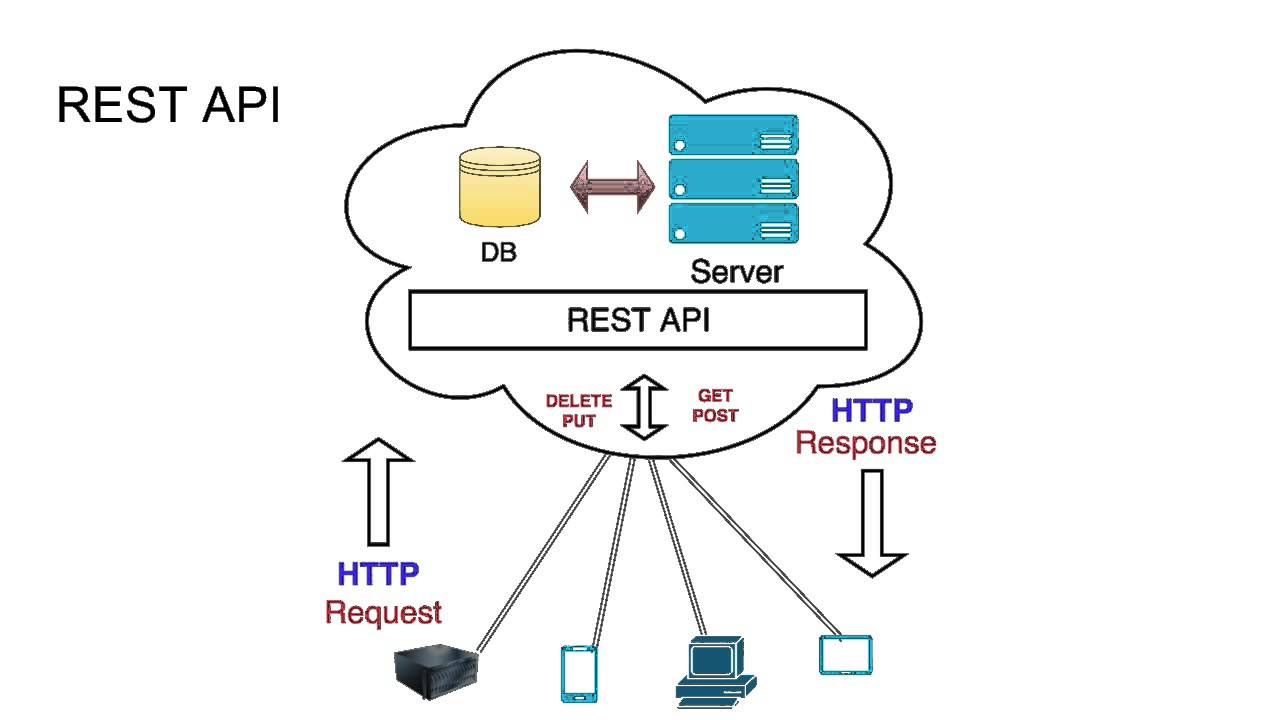
\includegraphics[height=6cm,width=1\textwidth,keepaspectratio]{rest.jpg}
            % \caption{caption_name}
            \label{fig:rest.jpg}
        \end{figure}
         \vspace*{-1.0cm}
        \begin{center}
        \footnotesize
        \begin{tabular}{@{}lll@{}}
        \toprule
        Method & Action & CRUD \\
        \midrule
        GET & Retrieve resource & Read \\
        POST & Create resource & Create \\
        PUT & Replace resource & Update \\
        PATCH & Partial update & Update \\
        DELETE & Remove resource & Delete \\
        \bottomrule
        \end{tabular}
        \end{center}
    \end{column}
\end{columns}
\end{frame}

\begin{frame}[t]{REST API — Tasklist Example}
\framesubtitle{Mapping HTTP routes to CRUD operations}
\vspace{-0.2cm}
\begin{center}
\footnotesize
\begin{tabular}{@{}llp{6cm}@{}}
\toprule
\textbf{Route} & \textbf{Method} & \textbf{Action} \\
\midrule
\texttt{/tasks} & GET & Return list of all tasks \\
\texttt{/tasks} & POST & Create a new task \\
\texttt{/tasks/\{id\}} & GET & Return a single task by ID \\
\texttt{/tasks/\{id\}} & PUT & Replace the task with new data \\
\texttt{/tasks/\{id\}} & PATCH & Update selected fields of the task \\
\texttt{/tasks/\{id\}} & DELETE & Delete the task \\
\bottomrule
\end{tabular}
\end{center}
\vspace{3mm}

{URL identifies \emph{what} resource; HTTP method identifies \emph{what to do} with it.}
\end{frame}

\begin{frame}[t]{Python \texttt{requests} Library}
\framesubtitle{Making HTTP requests from Python}
        \textbf{Key features}
        \begin{itemize}
            \item One function per HTTP method: \texttt{requests.get()}, \texttt{.post()}, \texttt{.put()}, \texttt{.delete()}, \ldots
            \item Response object: \texttt{resp.status\_code}, \texttt{resp.headers}, \texttt{resp.json()}, \texttt{resp.content}
            \item Raise exception on bad status: \texttt{resp.raise\_for\_status()}
            \item \texttt{requests.Session()} — reuses TCP connection, shares headers/cookies
            \item Streaming downloads: \texttt{stream=True} + \texttt{iter\_content()}
        \end{itemize}
        \vspace{2mm}
        \textbf{Testing endpoints}
        \begin{itemize}
            \item \href{https://httpbin.org}{httpbin.org} — echoes your request back
            \item \href{https://jsonplaceholder.typicode.com}{jsonplaceholder.typicode.com} — fake REST data
        \end{itemize}

\end{frame}

% ---------------------------------------------------------------
% PART 3: FASTAPI
% ---------------------------------------------------------------
\begin{frame}[t]{What Is FastAPI?}
\vspace*{-0.4cm}
\begin{columns}[T,onlytextwidth]
    \begin{column}{0.56\textwidth}
        \textbf{FastAPI} is a Python web framework for building REST APIs quickly:
        \begin{itemize}
            \item \textbf{Decorator-based routing}: \texttt{@app.get("/items")}
            \item \textbf{Automatic data validation} via Pydantic models
            \item \textbf{Auto-generated docs}: Swagger UI at \texttt{/docs}
            \item \textbf{Async support} out of the box (\texttt{async def})
            \item Among the \textbf{fastest} Python frameworks (comparable to Node.js)
        \end{itemize}
        \vspace{3mm}
        {FastAPI = \textbf{Flask-like simplicity} + \textbf{async performance} + \textbf{automatic OpenAPI docs}}
    \end{column}
    \begin{column}{0.42\textwidth}
        \begin{figure}[H]
            \centering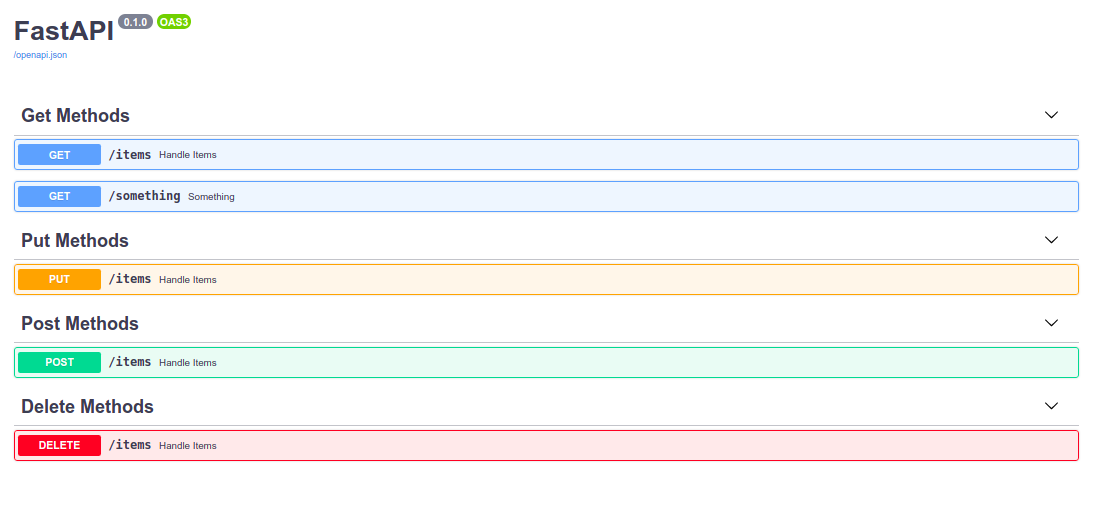
\includegraphics[height=6cm,width=1\textwidth,keepaspectratio]{svag.png}
            % \caption{caption_name}
            \label{fig:svag.png}
        \end{figure}
    \end{column}
\end{columns}
\end{frame}

\begin{frame}[t]{Building a REST Server with FastAPI}
\framesubtitle{Core concepts}
        \textbf{Application structure}
        \begin{itemize}
            \item Create an \texttt{FastAPI()} app instance
            \item Define \textbf{route handlers} with decorators
            \item Use \textbf{path parameters} (\texttt{/items/\{id\}}) and \textbf{query parameters}
            \item Use \textbf{Pydantic models} to declare request/response schemas
            \item Run with \texttt{uvicorn app:app --reload}
        \end{itemize}
        \vspace{3mm}
        \textbf{Request body vs.~query string}
        \begin{itemize}
            \item Query string: simple scalars in the URL
            \item Request body: structured JSON (POST/PUT/PATCH)
        \end{itemize}
\end{frame}

\begin{frame}[t]{FastAPI — Request Lifecycle}
\framesubtitle{From HTTP bytes to Python and back}
\vspace{-0.2cm}
\begin{center}
\begin{tikzpicture}[
    box/.style={draw, rounded corners=3pt, minimum width=2.4cm, minimum height=0.7cm, align=center, font=\small},
    arr/.style={-Stealth, thick},
    node distance=0.4cm and 0.5cm
]
\node[box, fill=blue!15]  (client)  {Client\\(browser / script)};
\node[box, fill=green!15, right=1cm of client]  (uvicorn) {uvicorn\\ASGI server};
\node[box, fill=orange!15, right=1cm of uvicorn] (router)  {FastAPI\\Router};
\node[box, fill=red!15,    right=1cm of router]  (handler) {Handler\\function};
\node[box, fill=gray!15,   below=0.9cm of router] (valid)   {Pydantic\\validation};

\draw[arr] (client)   -- node[above,font=\footnotesize]{HTTP req} (uvicorn);
\draw[arr] (uvicorn)  -- node[above,font=\footnotesize]{route} (router);
\draw[arr] (router)   -- node[above,font=\footnotesize]{call} (handler);
\draw[arr] (router)   -- node[right,font=\footnotesize]{validate} (valid);
\draw[arr] (handler.south) -- ++(0,-0.5) -| node[below,font=\footnotesize]{JSON response} (client.south);
\end{tikzpicture}
\end{center}
\vspace{2mm}
\begin{itemize}
    \item \textbf{uvicorn} — ASGI web server (like gunicorn for WSGI)
    \item \textbf{Pydantic} — validates and coerces input/output data types automatically
    \item \textbf{OpenAPI schema} generated automatically from type annotations
\end{itemize}
\end{frame}

\begin{frame}[t]{FastAPI vs.~Other Frameworks}
\framesubtitle{When to choose what}
\vspace{-0.1cm}
\begin{center}
\footnotesize
\begin{tabular}{@{}p{2.7cm}p{3.3cm}p{3.3cm}p{3.3cm}@{}}
\toprule
 & \textbf{Flask} & \textbf{Django REST} & \textbf{FastAPI} \\
\midrule
Paradigm & Sync (WSGI) & Sync (WSGI) & Async (ASGI) \\
Speed & Moderate & Moderate & High \\
Data validation & Manual & DRF serializers & Pydantic (auto) \\
API docs & None built-in & DRF browsable API & Swagger + ReDoc \\
Learning curve & Low & Medium & Low--Medium \\
Best for & Small services & Full Django projects & Modern APIs, ML serving \\
\bottomrule
\end{tabular}
\end{center}
\vspace{3mm}
{For AI/ML model serving FastAPI is the de-facto standard: lightweight, fast, and self-documenting.}
\end{frame}

% ---------------------------------------------------------------
% PART 4: GRADIO
% ---------------------------------------------------------------
\begin{frame}[t]{What Is Gradio?}
\begin{columns}[T,onlytextwidth]
    \vspace*{-0.5cm}
    \begin{column}{0.54\textwidth}
        \textbf{Gradio} is a Python library that turns any function into a shareable web app:
        \begin{itemize}
            \item Define your function
            \item Declare inputs and outputs as \textbf{components}
            \item Call \texttt{demo.launch()} — that is all
        \end{itemize}
        \vspace{2mm}
        \textbf{Under the hood}
        \begin{itemize}
            \item Gradio starts a local \textbf{FastAPI server}
            \item Your function is exposed as a REST endpoint
            \item A prebuilt React frontend
            \item \texttt{share=True} creates a public tunnel via HuggingFace
        \end{itemize}
    \end{column}
    \begin{column}{0.44\textwidth}
        \vspace*{-1cm}
        \begin{figure}[H]
            \centering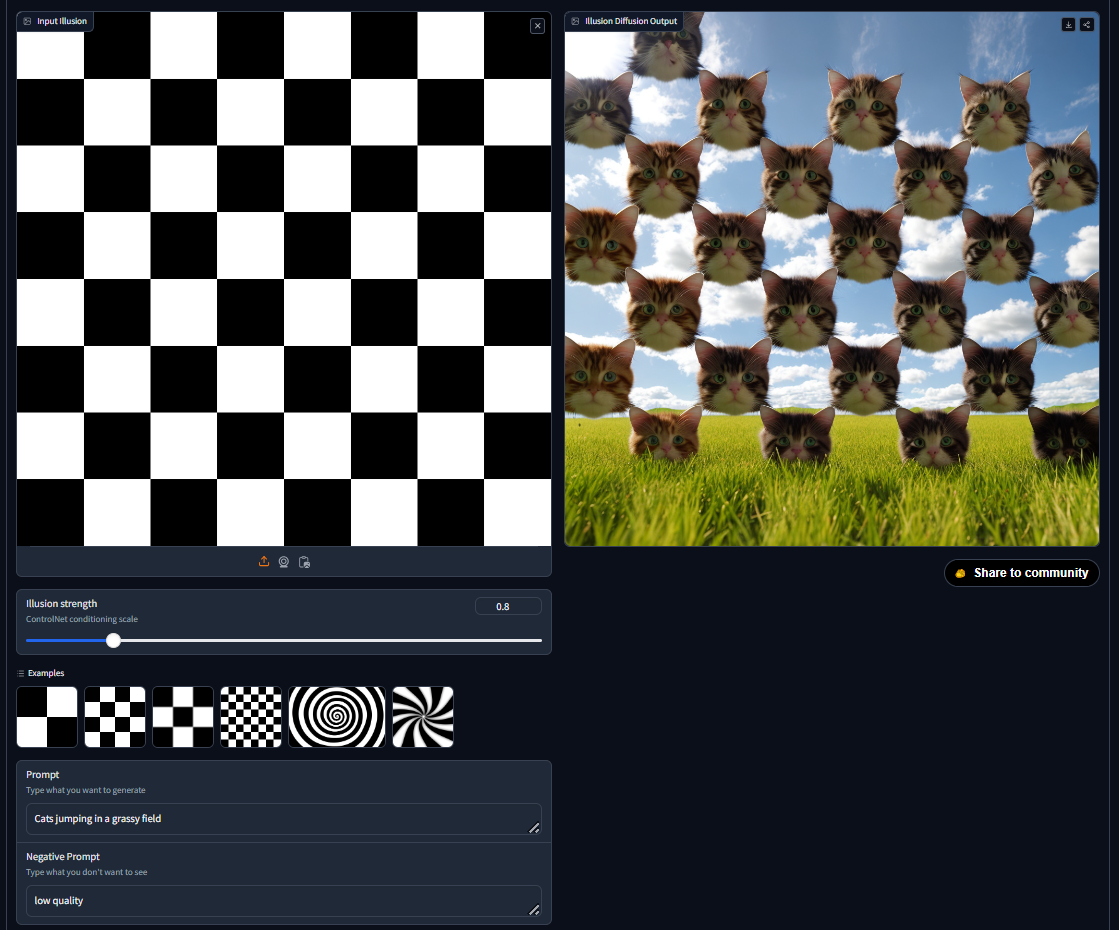
\includegraphics[height=6cm,width=1\textwidth,keepaspectratio]{Gradio_example.png}
            % \caption{caption_name}
            \label{fig:Gradio_example.png}
        \end{figure}
    \end{column}
\end{columns}
\end{frame}

\begin{frame}[t]{Gradio Components Cheatsheet}
\framesubtitle{Inputs and outputs for every modality}
\vspace{-0.2cm}
\begin{columns}[T,onlytextwidth]
    \begin{column}{0.49\textwidth}
        \textbf{Text \& numbers}
        \begin{itemize}
            \item \texttt{gr.Textbox()} — plain / multi-line text
            \item \texttt{gr.Number()} — numeric field
            \item \texttt{gr.Slider(min, max)} — range picker
        \end{itemize}
        \textbf{Choice}
        \begin{itemize}
            \item \texttt{gr.Radio(choices=[\ldots])}
            \item \texttt{gr.Dropdown(choices=[\ldots])}
            \item \texttt{gr.Checkbox()}
        \end{itemize}
        \textbf{Media}
        \begin{itemize}
            \item \texttt{gr.Image(type=\textquotedbl pil\textquotedbl)}
            \item \texttt{gr.Audio()}, \texttt{gr.Video()}
            \item \texttt{gr.File()}
        \end{itemize}
    \end{column}
    \begin{column}{0.49\textwidth}
        \textbf{Display}
        \begin{itemize}
            \item \texttt{gr.Label()} — classification result
            \item \texttt{gr.Dataframe()} — table
            \item \texttt{gr.Markdown()}, \texttt{gr.HTML()}
        \end{itemize}
        \vspace*{-1.0cm}
        \begin{figure}[H]
            \centering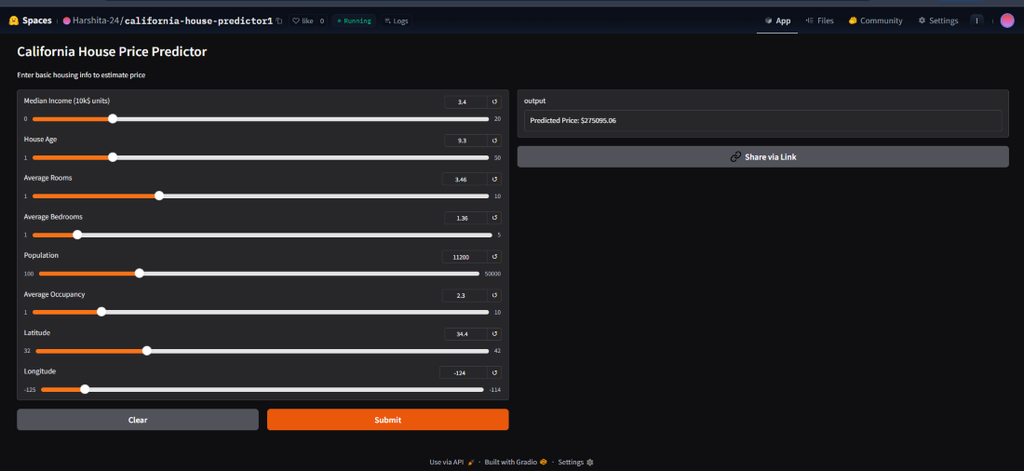
\includegraphics[height=6cm,width=1\textwidth,keepaspectratio]{gradio_widgets.png}
            % \caption{caption_name}
            \label{fig:gradio_widgets.png}
        \end{figure}
    \end{column}
\end{columns}
\end{frame}

\begin{frame}[t]{\texttt{gr.Interface} vs.~\texttt{gr.Blocks}}
\framesubtitle{Two levels of layout control}
\begin{columns}[T,onlytextwidth]
    \begin{column}{0.49\textwidth}
        \textbf{gr.Interface} — simple wrapper
        \begin{itemize}
            \item Pass \texttt{fn}, \texttt{inputs}, \texttt{outputs}
            \item Generates a standard two-column layout automatically
            \item Good for quick demos and single-function apps
        \end{itemize}

    \end{column}
    \begin{column}{0.49\textwidth}
\textbf{gr.Blocks} — full control
        \begin{itemize}
            \item Place components in rows/columns manually
            \item Bind \textbf{multiple events}: \texttt{.click()}, \texttt{.change()}, \texttt{.submit()}
            \item Multiple inputs/outputs per event
            \item Multi-step or multi-model pipelines
        \end{itemize}
    \end{column}
\end{columns}
\end{frame}

\begin{frame}[t]{Gradio + HuggingFace Models}

\begin{columns}[T,onlytextwidth]
    \vspace*{-0.4cm}
    \begin{column}{0.52\textwidth}
        \textbf{Pattern}
        \begin{enumerate}
            \item Load model with \texttt{transformers.pipeline(\ldots)}
            \item Write a thin wrapper function
            \item Wrap with \texttt{gr.Interface(fn=wrapper, \ldots)}
            \item Call \texttt{.launch()}
        \end{enumerate}
        \vspace{3mm}
        \textbf{Available tasks out of the box}
        \begin{itemize}
            \item Sentiment analysis, text generation
            \item Image classification, object detection
            \item Speech recognition, translation
        \end{itemize}
    \end{column}
    \begin{column}{0.46\textwidth}
        \begin{figure}[H]
            \centering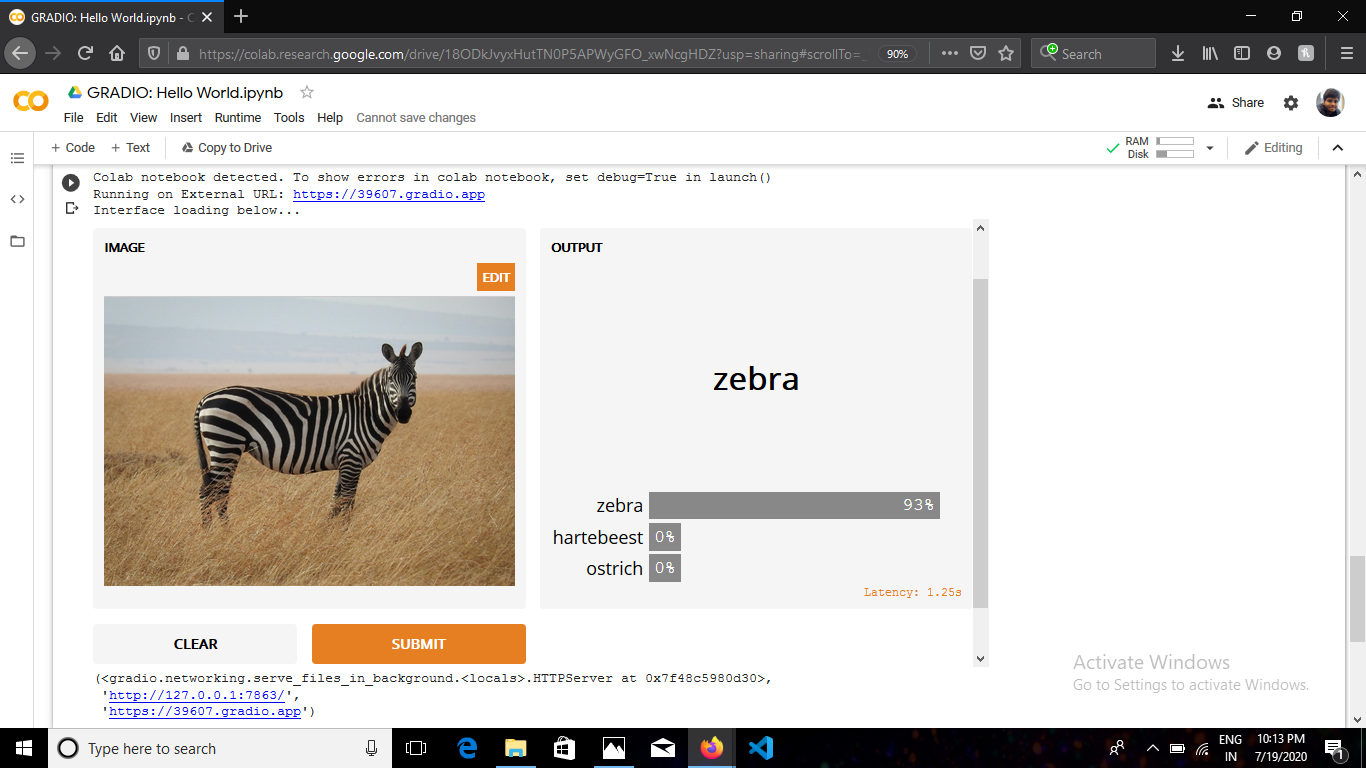
\includegraphics[height=6cm,width=1\textwidth,keepaspectratio]{gradio.png}
            % \caption{caption_name}
            \label{fig:gradio.png}
        \end{figure}
    \end{column}
\end{columns}
\end{frame}

\begin{frame}[t]{Putting It Together}
\framesubtitle{Model serving architecture — two approaches}
\vspace{-0.2cm}
\begin{columns}[T,onlytextwidth]
    \begin{column}{0.49\textwidth}
        \textbf{Approach A: FastAPI only}
        \begin{itemize}
            \item \texttt{POST /predict} accepts JSON, returns JSON
            \item Frontend is separate (React, mobile app, \ldots)
            \item Best for production APIs consumed by other services
        \end{itemize}

    \end{column}
    \begin{column}{0.49\textwidth}
        \textbf{Approach B: Gradio only}
        \begin{itemize}
            \item One Python file, instant UI + API
            \item Built-in REST endpoint at \texttt{/api/predict}
            \item Best for demos, research, rapid prototyping
        \end{itemize}
        \textbf{Approach C: FastAPI + Gradio mounted together}
        \begin{itemize}
            \item Gradio app mounted into FastAPI via \texttt{app.mount()}
            \item One server, both UI and API routes
        \end{itemize}
    \end{column}
\end{columns}
\end{frame}

\begin{frame}[t]{Summary}
 \vspace*{-0.7cm}
\begin{columns}[T,onlytextwidth]
    \begin{column}{0.54\textwidth}
        \footnotesize
        \begin{itemize}
            \item \textbf{TCP/IP \& HTTP}: how clients and servers talk — request/response, methods, status codes, headers
            \item \textbf{REST API}: uniform interface for resources using HTTP — GET/POST/PUT/PATCH/DELETE mapped to CRUD
            \item \textbf{Python \texttt{requests}}: consuming REST APIs from Python
            \item \textbf{FastAPI}: building REST servers — routing, Pydantic validation, auto-docs, async
            \item \textbf{Gradio}: wrapping any Python function in a web UI — components, Interface vs.\ Blocks, HuggingFace integration
        \end{itemize}
    \end{column}
    \begin{column}{0.44\textwidth}
        \textbf{Extra material (notebooks)}
        \begin{itemize}
            \item \texttt{rest\_api\_example.ipynb}\\ TCP/IP stack, HTTP deep dive, \texttt{requests} library with GET/POST/PUT/PATCH/DELETE examples
            \item \texttt{gradio\_example.ipynb}\\ Hello World, components, Blocks, model integration (sentiment, image classification)
        \end{itemize}
    \end{column}
\end{columns}
\end{frame}

\begin{frame}[t]{References}
\framesubtitle{}
    \begin{itemize}
        \item \href{https://www.youtube.com/playlist?list=PL6xV3OpvkyrjKvi2YfQlba93WrGb38c5L}{Fast API Tutorial (playlist)}
        \item \href{https://www.youtube.com/watch?v=-mN3VyJuCjM}{What is REST API?}
        \item \href{https://www.youtube.com/watch?v=mkpJIZWQlHY}{Что такое REST API?}
        \item \href{https://youtu.be/ABNxNFPqIGQ?si=fck41qw8f_odl7wv}{LLM app based on Gradio}
    \end{itemize}
\end{frame}

\fbckg{fibeamer/figs/last_page.png}
\frame[plain]{}

\end{document}
